%==============================================================================
% locality-approach.tex
%==============================================================================

\chapter{Approach}
\label{chap:locality-approach}

As a motivating example we implement a synthetic multi-threaded
locality-aware benchmark called \emph{Cache Stress Test}. 

If a multi-threaded benchmark with best possible locality has better
performance and fewer last-level cache misses than the same benchmark
with another or no specific locality, we should be able to see the
same effect when porting the benchmark to a locality-aware
implementation of intervals. Hence, we know whether it makes sense to
design a locality-aware intervals scheduler.

We wrote our benchmark for the Intel Nehalem system introduced in
Appendix \ref{sec:experimental-setup-mafushi}. The system has two
processors with totally 8 cores. While every core has its separate
level 1 and level 2 caches, the per-processor 8 MB level 3 cache is
shared between all cores of the same processor.

\emph{Cache Stress Test} first randomly initializes two integer arrays
of size \numprint{2097144}. Thus, the size of each array is about 8
MB, which is the same as the size of the last level cache per
processor. Then the benchmark creates 64 threads with their affinity
set to a specific processor: 32 have an affinity for the first
processor and 32 for the second processor. Section describes
\ref{sec:locality-implementation-core-affinity} our methodology of
binding Java threads to specific processing units.

One half of the threads operates on the elements of the first array
and the other half operates on the elements of the second array. Each
thread adds and multiplies all the elements of its respective array
100 times.

We implement several different variants of the \emph{Cache Stress
  Test}:

\begin{itemize}
\item \emph{Best Locality:} All the threads working on the first array
  have affinity for the first processor and all threads working on the
  second array have affinity for the second processor.
\item \emph{Ignorant Locality:} The threads are not bound to any
  specific processor, i.e. they are \emph{ignorant} of their locality.
\item \emph{Random Locality:} The affinity of the threads is set to a
  \emph{random} processor.
\item \emph{Worst Locality:} Half the threads with affinity for the
  first processor work on the first array, and the other half works on
  the second array and vice versa.
\end{itemize}

In the variant with \emph{best locality}, the first threads executing
warm up the cache by bringing in the elements of the array. Following
threads can get the array elements from the level 3 cache instead
from the main memory.

In the other variants, the elements in the cache might be overwritten
when a thread tries to access elements of an array which are not
cached already or the thread has to fetch them from the L3 cache of
the other processor.

Table \ref{tab:locality-approach-cache-stress-test} shows the
execution times and the speedups over the sequential algorithm for the
different locality implementations. As expected, the implementation
with \emph{best locality} is the fastest and provides the best
speedup. 

\begin{table}[htb]
  \centering
  \begin{tabular}{ln{2}{3}n{1}{2}}
    \toprule
    & {Runtime (in seconds)} & {Speedup (over sequential)} \\\midrule
    \emph{Best Locality} & 3.327 & 7.69 \\
    \emph{Ignorant Locality} & 3.985 & 6.42 \\
    \emph{Random Locality} & 5.175 & 5.83 \\
    \emph{Worst Locality} & 4.389 & 4.94 \\
    \emph{Sequential Implementation}\hspace{0.5cm} & 25.571 & 1 \\\bottomrule
  \end{tabular}
  \caption{Multi-threaded \emph{Cache Stress Test} execution times and speedups over sequential implementation}
  \label{tab:locality-approach-cache-stress-test}
\end{table}

Figure \ref{fig:locality-approach-cache-stress-test} illustrates the
execution times normalized to that of the \emph{best locality}
implementation. The \emph{best locality} implementation shows a
significant speedup over the other locality benchmarks of
1.2\texttimes\ -- 1.55\texttimes.

\begin{figure}[!ht]
  \centering
  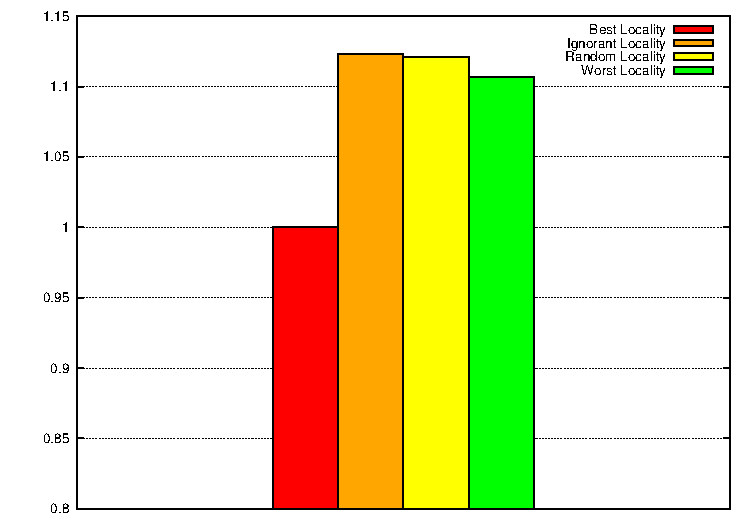
\includegraphics[width=0.7\linewidth]{locality-approach/cache-stress-test}
  \caption{Multi-threaded \emph{Cache Stress Test} with execution
    times normalized to \emph{best locality}}
  \label{fig:locality-approach-cache-stress-test}
\end{figure}

We measure the cache misses with perfmon2 \cite{Eranian2008} to check
whether our hypothesis is correct. 

Table \ref{tab:locality-approach-cache-stress-test} lists the number
of L3 cache read misses and hits. In Figure
\ref{fig:locality-approach-cache-stress-test} they are shown
normalized to the measurements of the \emph{best locality}
implementation. The \emph{best locality} benchmark has between
3.6\texttimes\ and 4.5\texttimes\ fewer L3 cache read misses than the
other benchmarks. Compared to the other benchmarks, it has between
1.5\texttimes\ and 1.8\texttimes\ more L3 cache read hits.

\todo{Add reference to ``Performance -> Methodology''}

\begin{table}[htb]
  \centering
  \begin{tabular}{ln{4}{0}n{4}{0}}
    \toprule
    & {L3 Cache Read Misses} & {L3 Cache Read Hits} \\\midrule
    \emph{Best Locality}\hspace{1cm} & 220 & 260 \\
    \emph{Ignorant Locality} & 800 & 170 \\
    \emph{Random Locality} & 900 & 165 \\
    \emph{Worst Locality} & 1000 & 140 \\\bottomrule
  \end{tabular}
  \caption[Multi-threaded \emph{Cache Stress Test} L3 cache read misses and hits]
  {Multi-threaded \emph{Cache Stress Test} L3 cache read misses and hits (rounded to the nearest million)}
  \label{tab:locality-approach-cache-stress-test}
\end{table}

\begin{figure}[!ht]
  \centering
  \subfloat[L3 Cache Read Misses]{
    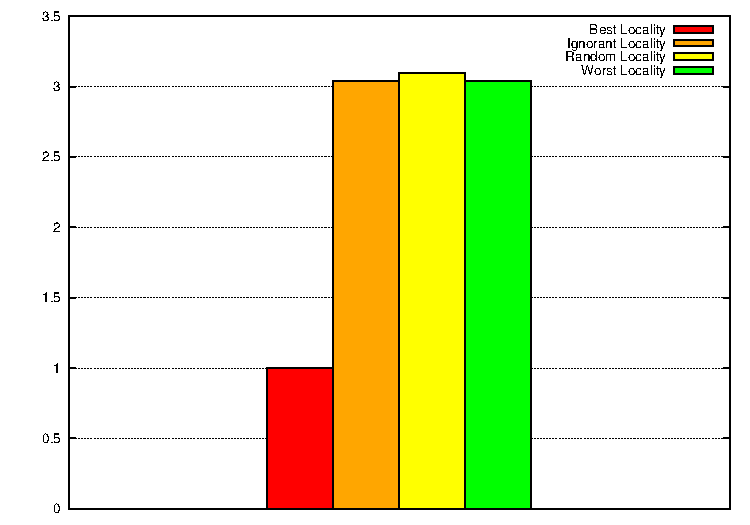
\includegraphics[width=0.5\linewidth]{locality-approach/cache-stress-test-cache-misses}
    \label{fig:locality-approach-cache-stress-test-cache-misses}
  }
  \subfloat[L3 Cache Read Hits]{
    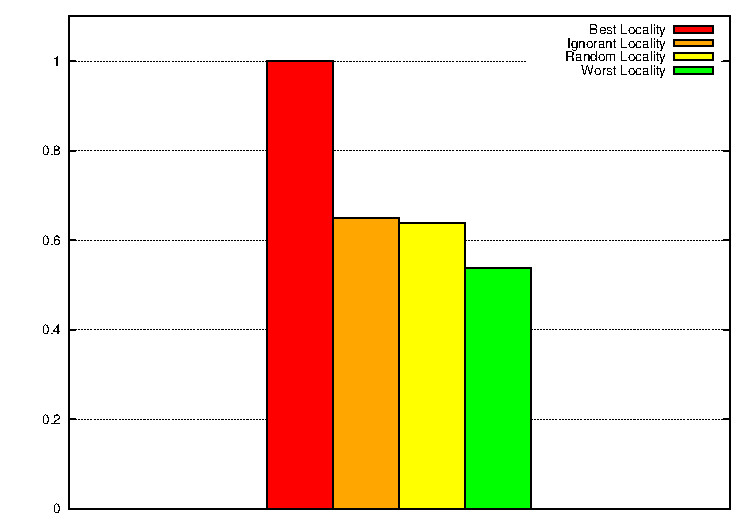
\includegraphics[width=0.5\linewidth]{locality-approach/cache-stress-test-cache-hits}
    \label{fig:locality-approach-cache-stress-test-cache-hits}
  }
  \caption{Multi-threaded \emph{Cache Stress Test} with L3 cache read
    misses and hits normalized to \emph{best locality}}
  \label{fig:locality-approach-cache-stress-test-cache}
\end{figure}

Our experiment confirmed our hypothesis that locality matters and we
decided to rewrite the intervals scheduler to support locality hints
provided by the programmer. Chapter \ref{chap:locality-implementation}
describes the implementation of the locality-aware scheduler. In
Chapter \ref{chap:locality-performance} we evaluate the performance of
the new scheduler implementation.


%%% Local Variables: 
%%% mode: latex
%%% TeX-master: "thesis"
%%% End: 